\chapter{Team Models}\label{chapter:team_model}

This section will investigate different models.

\section{Dixon and Coles}
The Dixon and Coles model is one developed for English football that uses full-time scores to predict the probabilities of a future match.  The following will be a deeper look into the football model with modifications made for basketball.

\subsection{Model}

The main assumption of the model is that the goals scored by the home and away team are independent Poisson variables.  The Poisson means in a particular game are determined by each team's attack and defence abilities.   In a match between teams $i$ and $j$, the number of goals scored by the home and away teams are denoted by

$$X_{ij} \sim \text{Poisson}(\alpha_i\beta_j\gamma),$$
$$Y_{ij} \sim \text{Poisson}(\alpha_j\beta_i),$$

where $X_{ij}$ and $Y_{ij}$ are independent, $\alpha_i, \beta_i > 0.$

Dixon and Coles present the following to determine the probabilities of goals scored in a match.

\begin{equation}\label{eq:base_dc}
\text{Pr}(X_{ij}=x, Y_{ij} = y) = \tau_{\lambda,\mu}(x, y)\frac{\lambda^x\exp(-\lambda)}{x!}\frac{\mu^y\exp(-\mu)}{y!}
\end{equation}

where

$$\lambda = \alpha_i\beta_j\gamma,$$
$$\mu = \alpha_j\beta_i,$$

and

\[
	\tau_{\lambda,\mu}(x,y) = 
	\begin{cases}
		1 - \lambda \mu \rho & \text{if } x=y=0,\\
		1 + \lambda \rho & \text{if } x=0,y=1,\\
		1 + \mu \rho & \text{if } x=1,y=0,\\
		1 - \rho & \text{if } x=1,y=1,\\
		1 & \text{otherwise}.
	\end{cases}
\]	



\subsection{Parameter Estimation}
Dixon and Coles imposed the following constraint to prevent the model from being overparameterized

$$\frac{1}{n}\sum_{i=1}^{n}\alpha_i = 1$$

For the National Basketball Association, there are 30 teams, which gives a total of 61 parameters to be estimated.  To estimate these parameters, a likelihood function is used.  For matches, $k=1,\ldots,N$, with scores $(x_k, y_k)$:

\begin{equation}\label{eq:dc_likelhiood}
L_t(\alpha_i, \beta_i,\gamma,i=1,\ldots,n) = \prod_{k=1}^{N} \exp(-\lambda_k)\lambda_{k}^{x_k}\exp(-\mu_k)
\end{equation}

where

$$\lambda_k = \alpha_{i(k)}\beta_{j(k)}\gamma,$$
$$\mu_k = \alpha_{j(k)}\beta_{i(k)},$$

and $i(k)$ and $j(k)$ are the indices of the home and away teams playing in match $k$.  The parameters can be found by maximising (\ref{eq:dc_likelhiood}).

\subsection{Model Limitation and Modification}
The basic limitation of model (\ref{eq:dc_likelhiood}) is that the parameters are static.  All the matches are weighed equally which leads to teams having the same ability parameters over time, when in reality team performance tends to fluctuate.  Especially over the course of multiple seasons where players may change teams.  Teams may go through multiple injuries, winning and losing streaks and multiple other factors.  The current model does not accurately reflect teams' recent form.  In order to compensate for this, Dixon and Coles introduced a modification to the model by adding a factor that will reduce the significance of older matches:

\begin{equation}\label{eq:dc_time}
L_t(\alpha_i, \beta_i,\gamma,i=1,\ldots,n) = \prod_{k=1}^{N} \{\exp(-\lambda_k)\lambda_{k}^{x_k}\exp(-\mu_k)\}^{\phi(t-t_k)}
\end{equation}

In the model, $t$ is the time the estimation was made and $t_k$ is the time match $k$ was played.  Match weighting can be changed by varying $\phi$.  Dixon and Coles chose the model

$$\phi(t) = \exp(-\xi t),$$

where all previous matches are downweighted exponentially based on $\xi > 0$.  When $\xi = 0$, all matches have equal weight, such as model (\ref{eq:dc_likelhiood}).  Larger values of $\xi$ will give more weight to recent matches.

Note that the probability of a home win in match $k$ is given by:

\begin{equation}\label{eq:prob}
p_k^H = \sum_\text{Pr}(X_{k} = x, Y_{k} = y)
\end{equation}

To optimise the selection of $\xi$.

\begin{equation}
S(\xi) = \sum_{k=1}^{N}(\delta_k^H\log p_k^H + \delta_k^A \log p_k^A)
\end{equation}

where, $\delta_k^H = 1$ if match $k$ was a home win and $\delta_k^H=0$ otherwise and vice versa for $\delta_k^A$.  The original model by Dixon and Coles includes a parameter for draws, but seeing as there are no draws in basketball it is ignored.  The function is maximised at $\xi=0.024$


\begin{figure}[!htb]
	\centering
	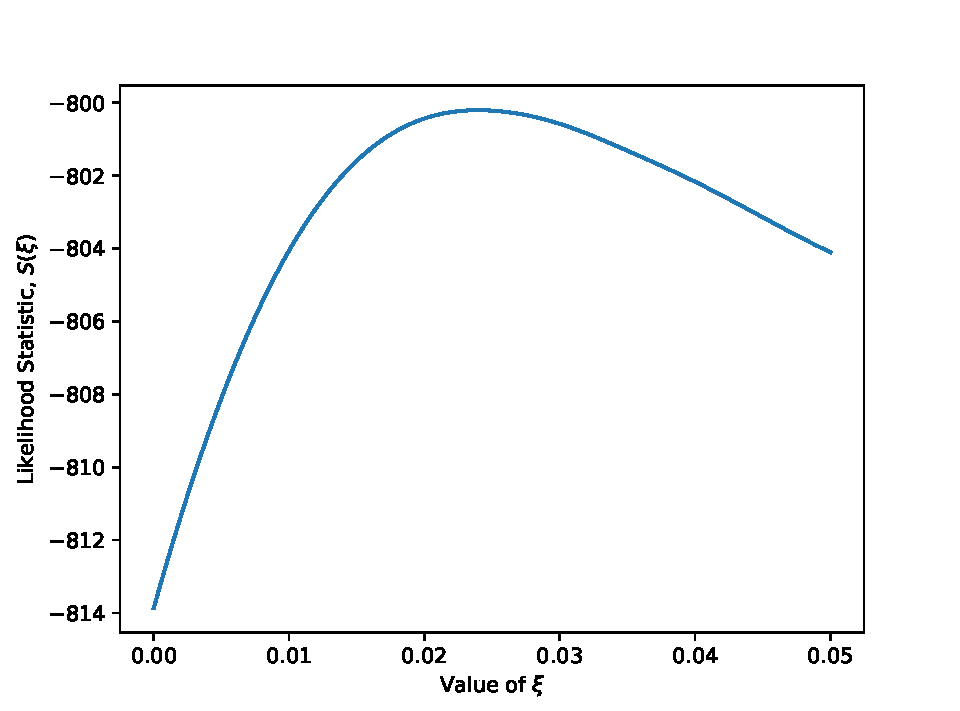
\includegraphics[width=0.75\textwidth]{{Figures/xi_plot.pdf}}
	\captionof{figure}{S($\xi$) vs $\xi$: The maximum occurs at $\xi = 0.024$.}
	\label{fig:xi}
\end{figure}



\subsection{Dynamic Parameter Estimation}
It seems that data from 1.5 seasons are required for the most accurate estimations.  Table \ref{table:dc} show the estimates on October 10th, 2016, splitting teams in the western and eastern conferences.  It is interesting to note that the Western Conference is clearly superior.

\begin{table}[!ht]
\centering

\begin{subtable}[t]{0.5\textwidth}\centering
	\begin{tabular}[t]{|l|c|c|}
		\hline
		\textbf{Team}  & \textbf{$\hat{\alpha}$} & \textbf{$\hat{\beta}$} \\ \hline
		Dallas Mavericks & 102.869 & 1.014 \\ \hline
		Denver Nuggets & 103.053 & 1.035\\ \hline
		Golden State Warriors & \textbf{106.907} & 1.002\\ \hline
		Houston Rockets & 105.584 & 1.024 \\ \hline
		Los Angeles Clippers & 104.276 & 0.982\\ \hline
		Los Angeles Lakers & 99.822 & 1.045 \\ \hline
		Memphis Grizzlies & 95.908 & 0.939\\ \hline
		Minnesota Timberwolves & 100.239 & 1.027\\ \hline
		New Orleans Pelicans & 98.449 & 1.003\\ \hline
		Oklahoma City Thunder & 105.840 & 0.995\\ \hline
		Phoenix Suns & 100.450 & 1.028\\ \hline
		Portland Trail Blazers & 102.473 & 1.007\\ \hline
		Sacramento Kings & 101.740 & 1.046\\ \hline
		San Antonio Spurs & 102.961 & \textbf{0.952}\\ \hline
		Utah Jazz & 95.716 & 0.966\\ \hline
		\textbf{Mean} & 101.752 & 1.004\\ \hline
	\end{tabular}
\caption{Western Conference}
\end{subtable}\hfill
\begin{subtable}[t]{0.5\textwidth}\centering
	\begin{tabular}[t]{|l|c|c|}
		\hline
		\textbf{Team}  & \textbf{$\hat{\alpha}$} & \textbf{$\hat{\beta}$} \\ \hline
		Atlanta Hawks  & 100.728 & 0.990\\ \hline
		Boston Celtics & 99.638 & 1.004\\ \hline
		Brooklyn Nets  & 97.690 & 1.004\\ \hline
		Charlotte Hornets & 96.624 & 0.994\\ \hline
		Chicago Bulls & 96.872 & 0.963\\ \hline
		Cleveland Cavaliers & 100.233 & 1.000\\ \hline
		Detroit Pistons & 98.845 & 1.012\\ \hline
		Indiana Pacers & 97.241 & \textbf{0.951} \\ \hline
		Miami Heat & 99.522 & 0.971\\ \hline
		Milwaukee Bucks & 97.573 & 1.012\\ \hline
		New York Knicks & 96.838 & 0.993\\ \hline
		Orlando Magic & 96.879 & 1.020\\ \hline
		Philadelphia 76ers & 95.337 & 1.036\\ \hline
		Toronto Raptors & \textbf{100.927} & 0.991 \\ \hline
		Washington Wizards & 98.768 & 0.994\\ \hline
		\textbf{Mean} & 98.248 & 0.996\\ \hline
	\end{tabular}
\caption{Eastern Conference}
\end{subtable}

\caption{lala}
\label{table:dc}

\end{table}

\begin{figure}[!ht]
	\centering
	\begin{subfigure}{0.67\linewidth}
	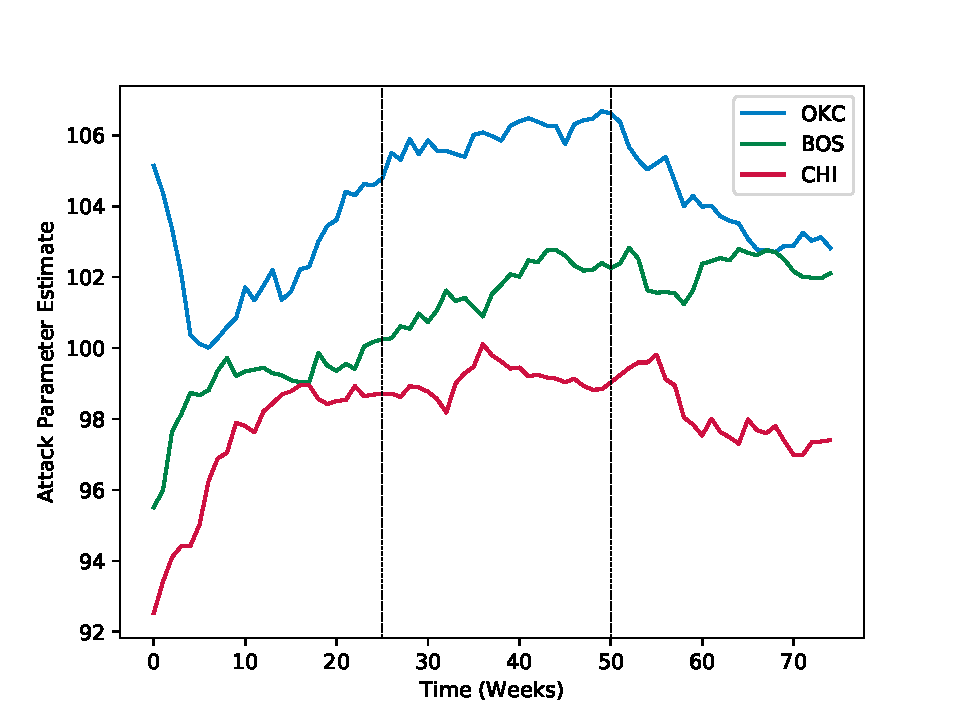
\includegraphics[width=1\textwidth]{{Figures/weeks_attack.pdf}}
	\caption{}	
	\end{subfigure}
	
	\begin{subfigure}{0.67\linewidth}
	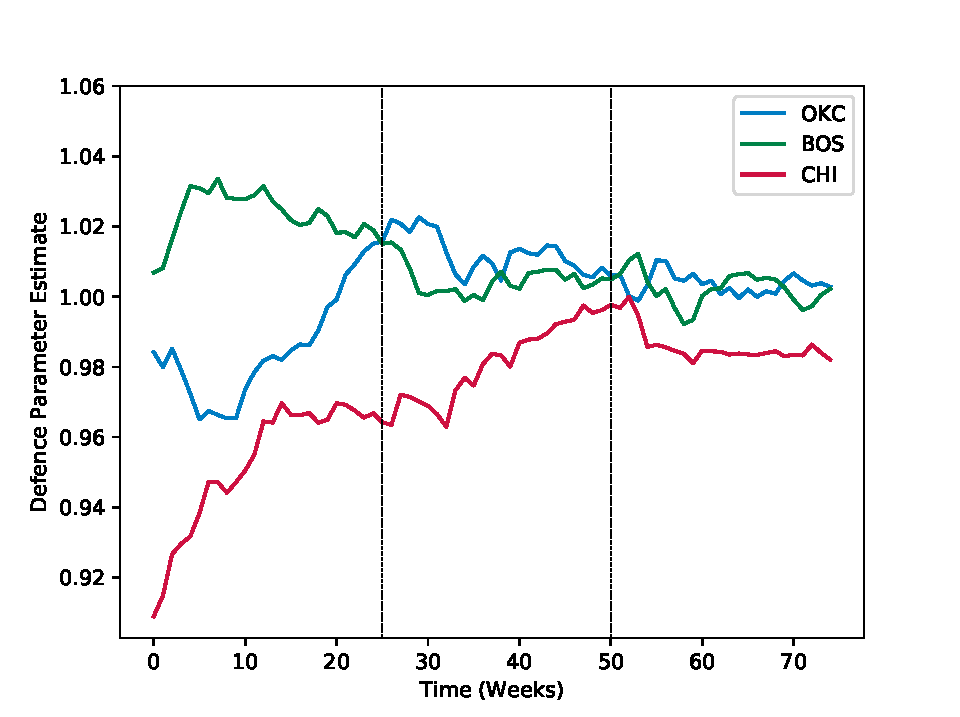
\includegraphics[width=1\textwidth]{{Figures/weeks_defence.pdf}}
	\caption{}
	\end{subfigure}
	
	\begin{subfigure}{0.67\linewidth}
	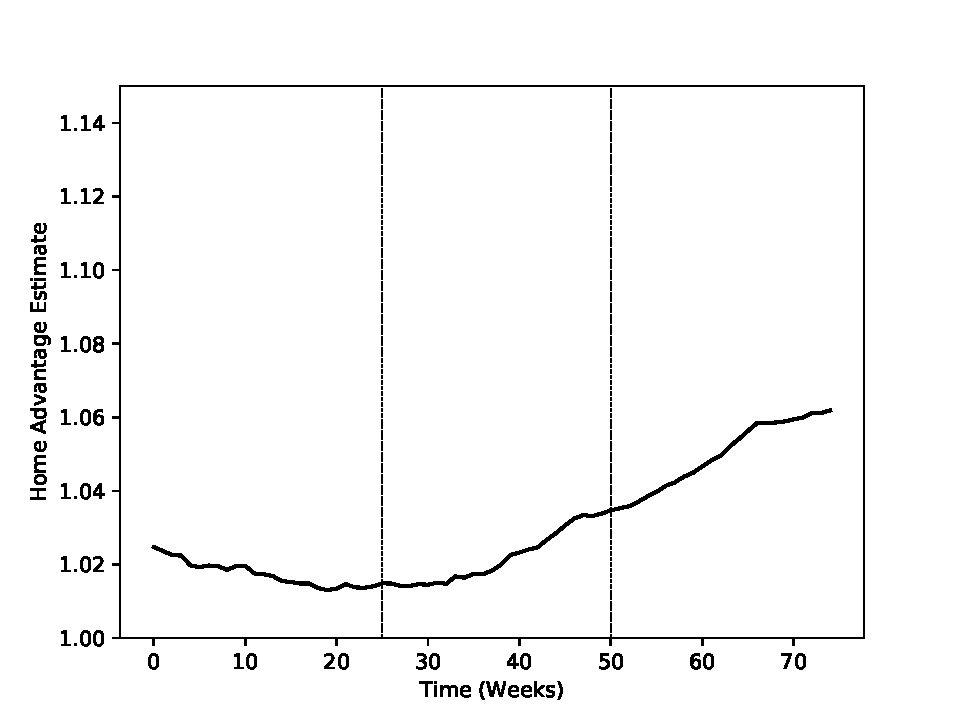
\includegraphics[width=1\textwidth]{{Figures/weeks_home.pdf}}
	\caption{}
	\end{subfigure}
	
	\caption{(A),(B) Attack and defence parameter weekly estimates for the Oklahoma City Thunder, Boston Celtics and Chicago Bulls; (C) Home advantage parameter variation.\label{fig:weeks_dc}}
	
	
\end{figure}

\section{Dixon and Robinson}
Dixon and Robinson began by extending model (\ref{eq:dc_likelhiood}) created by Dixon and Coles \citep{dixon_coles}.

\begin{equation}
\begin{split}
\lambda_k(t) & = \lambda_k = \alpha_{i(k)}\beta_{j(k)}\gamma, \\
\mu_k(t)  & = \mu_k = \alpha_{j(k)}\beta_{i(k)}
\end{split}
\end{equation}


\begin{equation}
(\bm{t}_k, \bm{J}_k) = \{(t_{k,l}, J_{k,l}: l=1,\ldots,m_k\}
\end{equation}

$$\lambda_k(t) = \lambda_{xy}\lambda_k$$

and

$$\mu_k(t) = \mu_{xy}\mu_k$$

\begin{equation}
    \lambda_t(k)= 
\begin{cases}
	\rho_1\lambda_{xy}\lambda_k,& \text{for }t \in(44/90, 45/90], \\
	\rho_2\lambda_{xy}\lambda_k,& \text{for }t \in(89/90, 90/90], \\
    \lambda_{xy}\lambda_k,      & \text{otherwise}
\end{cases}
\end{equation}

% Stoppage Time Parameters
Dixon and Robinson extended the model by introducing new parameters to represent goals scored during injury time (45+, 90+ minutes).  Figure \ref{fig:point_dist} is a histogram for the point times in games from the 2013-2016 seasons.  There appears to be more points scored at the end of each quarter, especially at the end of the game.  Thus, the basketball model will include the $\rho$ parameters.  However, it will include 4 parameters instead of 2 for each quarter.


\begin{figure}[!htb]
	\centering
	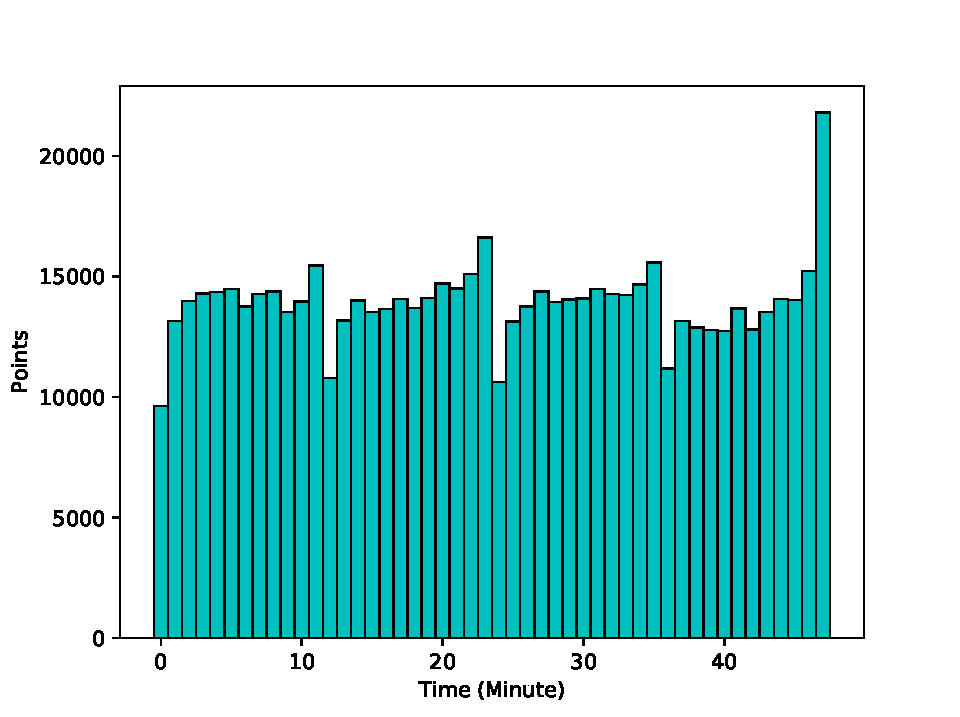
\includegraphics[width=0.75\textwidth]{{Figures/point_dist.pdf}}
	\captionof{figure}{Histogram of point times}
	\label{fig:point_dist}
\end{figure}

\begin{equation}
L(\bm{t}_k, \bm{J}_k) = \exp(-\bm{\wedge}[0, 1])\exp(-\text{\textbf{Y}}[0, 1])\prod_{l=1}^{m_k}\lambda_k(t_{k,l})^{1-J_{k,l}}\mu_k(t_{k,l})^{J_{k,l}}
\end{equation}

where

$$\bm{\wedge}[t_1, t_2] = \int_{t_1}^{t_2}\lambda_k(t)dt$$

and

$$\text{\textbf{Y}}[t_1, t_2] = \int_{t_1}^{t_2}\mu_k(t)dt$$

\section{Player Model}

\begin{equation}
L(\alpha, \beta | X) = \{ \}^{\phi(t-t_k)}
\end{equation}
